\section{Results}


\subsection{Depletion calculation time}

Using the regression models:
    CPU times: user 2 µs, sys: 2 µs, total: 4 µs
    Wall time: 8.58 µs


\subsection{U.S. \gls{UNF} inventory comparison}



\begin{table}[h]
    \centering
    \begin{tabular}{lrrr}
        \hline
        Metric & Data & Recipe & Prediction \\
        \hline
        $^{239}Pu$ mass [t] & 333.32 & 327.16 & 332.99\\
        $^{137}Cs$ mass [t] & 66.42 & 66.67 & 66.42\\
        $^{235}U$ mass [t] & 496.02 & 485.10 & 495.56\\
        Decay Heat [MW] & 201.25 & 183.79 & 201.29 \\
        Activity [Bq] & $2.91e21$ & $2.62e21$ & $2.91e21$ \\
        \hline
    \end{tabular}
    \caption{Comparison of \gls{PWR} \gls{UNF} inventory in the U.S.,
             using the Unified database.}
\end{table}


\begin{table}[h]
    \centering
    \begin{tabular}{lcrrr}
        \hline
        Metric & Year & HR case & Prediction case  & Error [\%] \\
        \hline
        \multirow{3}{*}{\shortstack{Decay \\ Heat}} & 2020 & 42.67 & 42.63 &  \\
                                                    & 2100 & 17.08 & 17.07 & \\
                                                    & 3100 & 3.26 & 3.25 & \\
        \hline
        \multirow{3}{*}{\shortstack{Activity}} & 2020 & 4.86e20 & 4.86e20 & \\
                                               & 2100 & 6.65e19 & 6.65e19 & \\
                                               & 3100 & 3.82e15 & 3.82e15 & \\
        \hline
    \end{tabular}
    \caption{Decay heat and radioactivity values and errors for years 2020, 2100, and 3100.}
    \label{tab:wm}
\end{table}

\begin{figure}
    \centering
    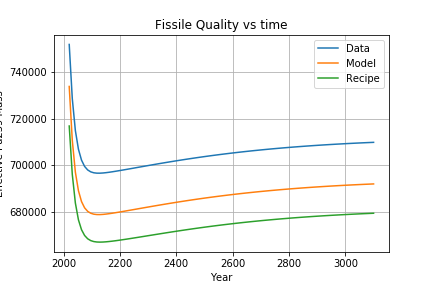
\includegraphics[width=\textwidth]{fiss.png}
    \caption{Effective Pu-239 mass value of \gls{UNF} inventory generated by
             Unifed database, average recipe, and the prediction model. }
    \label{fig:fiss}
\end{figure}

\begin{figure}
    \centering
    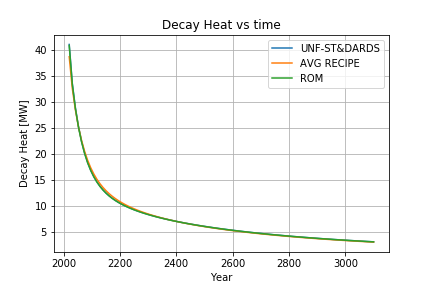
\includegraphics[width=\textwidth]{heat.png}
    \caption{Decay heat of \gls{UNF} inventory generated by
             Unifed database, average recipe, and the prediction model. }
    \label{fig:heat}
\end{figure}

\begin{figure}
    \centering
    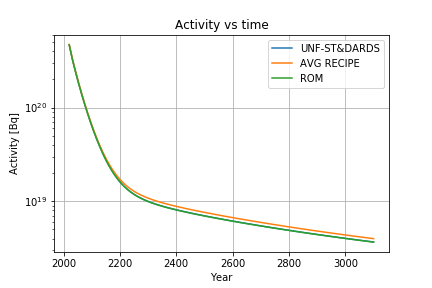
\includegraphics[width=\textwidth]{activity.png}
    \caption{Activity of \gls{UNF} inventory generated by
             Unifed database, average recipe, and the prediction model. }
    \label{fig:activity}
\end{figure}

\begin{figure}
    \centering
    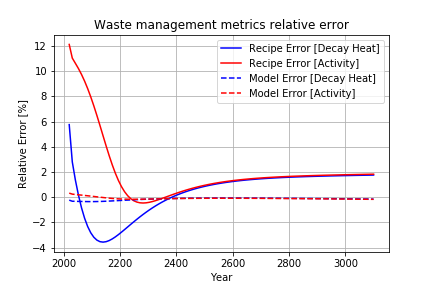
\includegraphics[width=\textwidth]{ha_err.png}
    \caption{Relative error of waste management metrics for \gls{UNF} inventory
             generated by the average recipe, and the prediction model.}
    \label{fig:ha_err}
\end{figure}


\subsection{SERPENT depletion comparison}

[andrei it's u bro]